\section{2021春}

\setcounter{yearcounter}{2021}
% \setcounter{page}{1}


\subsection{微分積分}
\prob{%
  以下の問いに答えよ。
  \begin{enumerate}[label=(\arabic*)]
    \item 次の関数$f(x)$を微分せよ。
    \begin{gather}
      f(x) = x^{x^x} \quad (x > 0)
    \end{gather}
    \item 次の極限値を求めよ。
    \begin{gather}
      \lim_{x\to +0}\left\{ \frac{1}{\log(1+x)} - \frac{1}{x} \right\}
    \end{gather}
  \end{enumerate}
}
% [?] なぜ極限が →+0 なのかわからない →0 でも同じ値に収束するはず
\begin{ans*}
  ${}$
  \begin{enumerate}[label=(\arabic*)]
    \item
    \begin{gather}
      g(x) = x^{x} \quad (x > 0)
    \end{gather}
    は\dm{\log g(x) = x\log x}より
    \begin{gather}
      \frac{g'(x)}{g(x)} = \log x + 1 \\
      \Rightarrow g'(x) = x^{x}(\log x + 1)
    \end{gather}

    $f(x)$の自然対数をとったものの微分は
    \begin{align}
      \frac{f'(x)}{f(x)}
      &= g'(x)\log x + \frac{g(x)}{x} \\
      &= x^{x}(\log x + 1) + x^{x-1} \\
      \therefore f'(x)
      &= x^{x^{x}}\Bigl(x^{x}(\log x + 1) + x^{x-1}\Bigr)
    \end{align}

    \item
    \begin{align}
      \lim_{x\to +0}\left\{ \frac{1}{\log(1+x)} - \frac{1}{x} \right\}
      = \lim_{x\to +0}\frac{x-\log(1+x)}{x\log(1+x)}
    \end{align}
    より$f(x) = x-\log(1+x),\,g(x) = x\log(1+x)$とおくと
    求める極限は
    \begin{gather}
      \lim_{x\to +0}\left\{ \frac{1}{\log(1+x)} - \frac{1}{x} \right\}
      = \lim_{x\to +0}\frac{f(x)}{g(x)}
    \end{gather}
    である。
    このとき導関数は
    \begin{align}
      f'(x) &= 1 - \frac{1}{1+x} \\
      f''(x)&= \frac{1}{(1+x)^2} \\
      g'(x) &= \log(1+x) + \frac{x}{1+x} \\
      g''(x)&= \frac{1}{1+x} + \frac{1}{1+x^2}
    \end{align}
    のように得られる。

    この二階導関数の極限は
    \begin{align}
      \lim_{x\to +0}\frac{f''(x)}{g''(x)}
      &= \lim_{x\to +0}\frac{\cfrac{1}{(1+x)^2}}{\cfrac{1}{1+x} + \cfrac{1}{1+x^2}} \\
      &= \frac{1}{2}
    \end{align}
    であり、$x=0$の除外近傍で\dm{g''(x) \neq 0}かつ
    \dm{
      \lim_{x\to +0} f'(x) = \lim_{x\to +0} g'(x) = 0
    }
    であるので\lhopital の定理より
    \begin{gather}
      \lim_{x\to +0}\frac{f'(x)}{g'(x)}
      =\frac{1}{2}
    \end{gather}
    同様に、$x=0$の除外近傍で\dm{g'(x)\neq 0}かつ
    \dm{
      \lim_{x\to +0}f(x) = \lim_{x\to +0}g(x) = 0
    }であるので\lhopital の定理より
    \begin{gather}
      \lim_{x\to +0}\frac{f(x)}{g(x)} = \frac{1}{2}
    \end{gather}
\end{enumerate}
\end{ans*}

\prob{%
  次の関数$f(x)$を考える。
  \begin{gather}
    f(x) = \frac{\gflr{x}}{x} \quad (0 < x < 3)
  \end{gather}
  ガウス記号$\gflr{x}$は床関数を表す。
  その値は実数$x$に対して$x$以下である最大の整数で与えられる。
  このとき、以下の問いに答えよ。
  \begin{enumerate}[label=(\arabic*)]
    \item $f(1/2),\,f(1),\,f(3/2)$の値を求めよ。
    \item 関数$f(x)$のグラフを描け。
  \end{enumerate}
}
\begin{ans*}
  ${}$
  \begin{enumerate}[label=(\arabic*)]
    \item
    \begin{align}
      f(1/2) &= 0 \\
      f(1) &= 1 \\
      f(3/2) &= \frac{4}{3}
    \end{align}
    \item $\gflr{x}=n\:(n\leq x < n+1)$より
    \begin{gather}
      f(x) =
      \begin{dcases}
        0 & (0 < x < 1) \\
        \frac{1}{x} & (1\leq x < 2) \\
        \frac{2}{x} & (2\leq x < 3)
      \end{dcases}
    \end{gather}

    \begin{figure}[H]\centering
      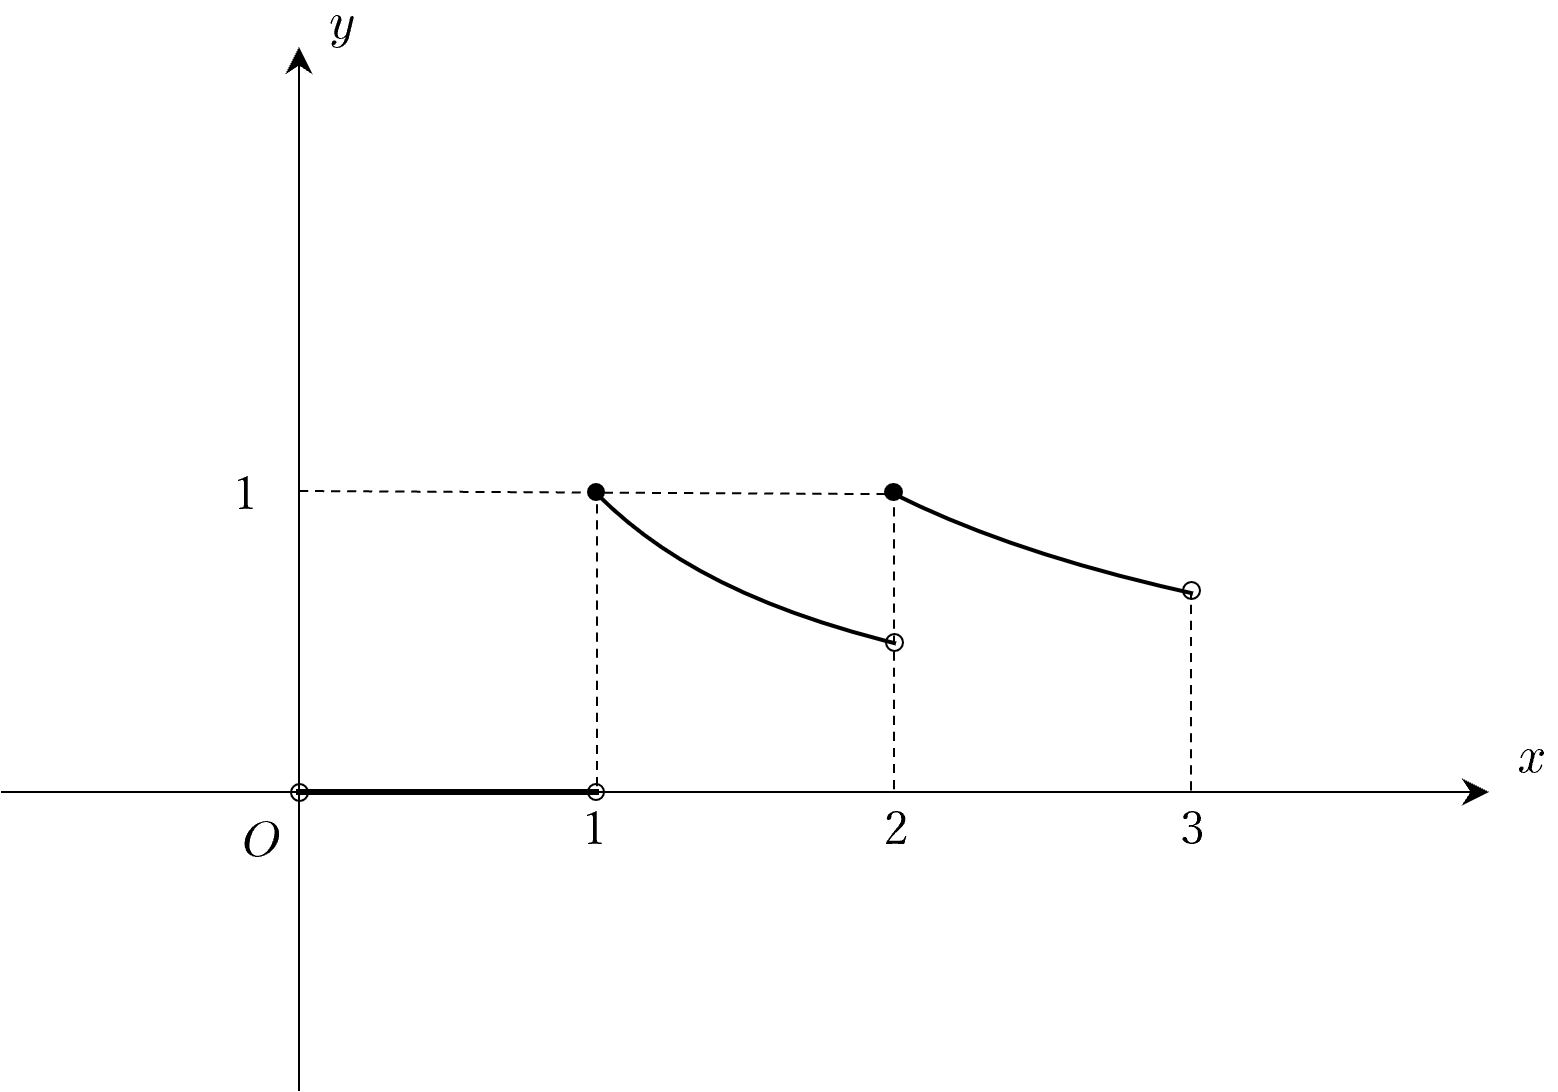
\includegraphics[width=.75\linewidth]{./src/fig/Basic/B_2021_spring_f.png}
    \end{figure}
  \end{enumerate}
\end{ans*}

\prob{
  次の重積分について、以下の問いに答えよ。
  \begin{gather}
    \iiint_D dxdydz,\quad
    D = \Dset{(x,y,z) \relmiddle
    x\geq 0,\,
    y\geq 0,\,
    z\geq 0,\,
    x^2+y^2+z^2\leq 1,\, x^2 + y^2 \leq x}
  \end{gather}
  \begin{enumerate}[label=(\arabic*)]
    \item 積分領域$D$を図示せよ。
    \item この重積分を計算せよ。
  \end{enumerate}
}
\begin{ans*}
  ${}$
  \begin{enumerate}[label=(\arabic*)]
    \item 略 % pic
    \item 与えられた領域$D$は$xy$平面を底面として
    球面までを高さとする立体であるので、\\
    積分領域\dm{D'=\Dset{(x,y)\relmiddle \biggl(x-\frac{1}{2}\biggr)^2+y^2\leq \frac{1}{4}}}において
    \dm{z = \sqrt{1-x^2-y^2}}を積分すれば良い。
    \begin{figure}[H]\centering
      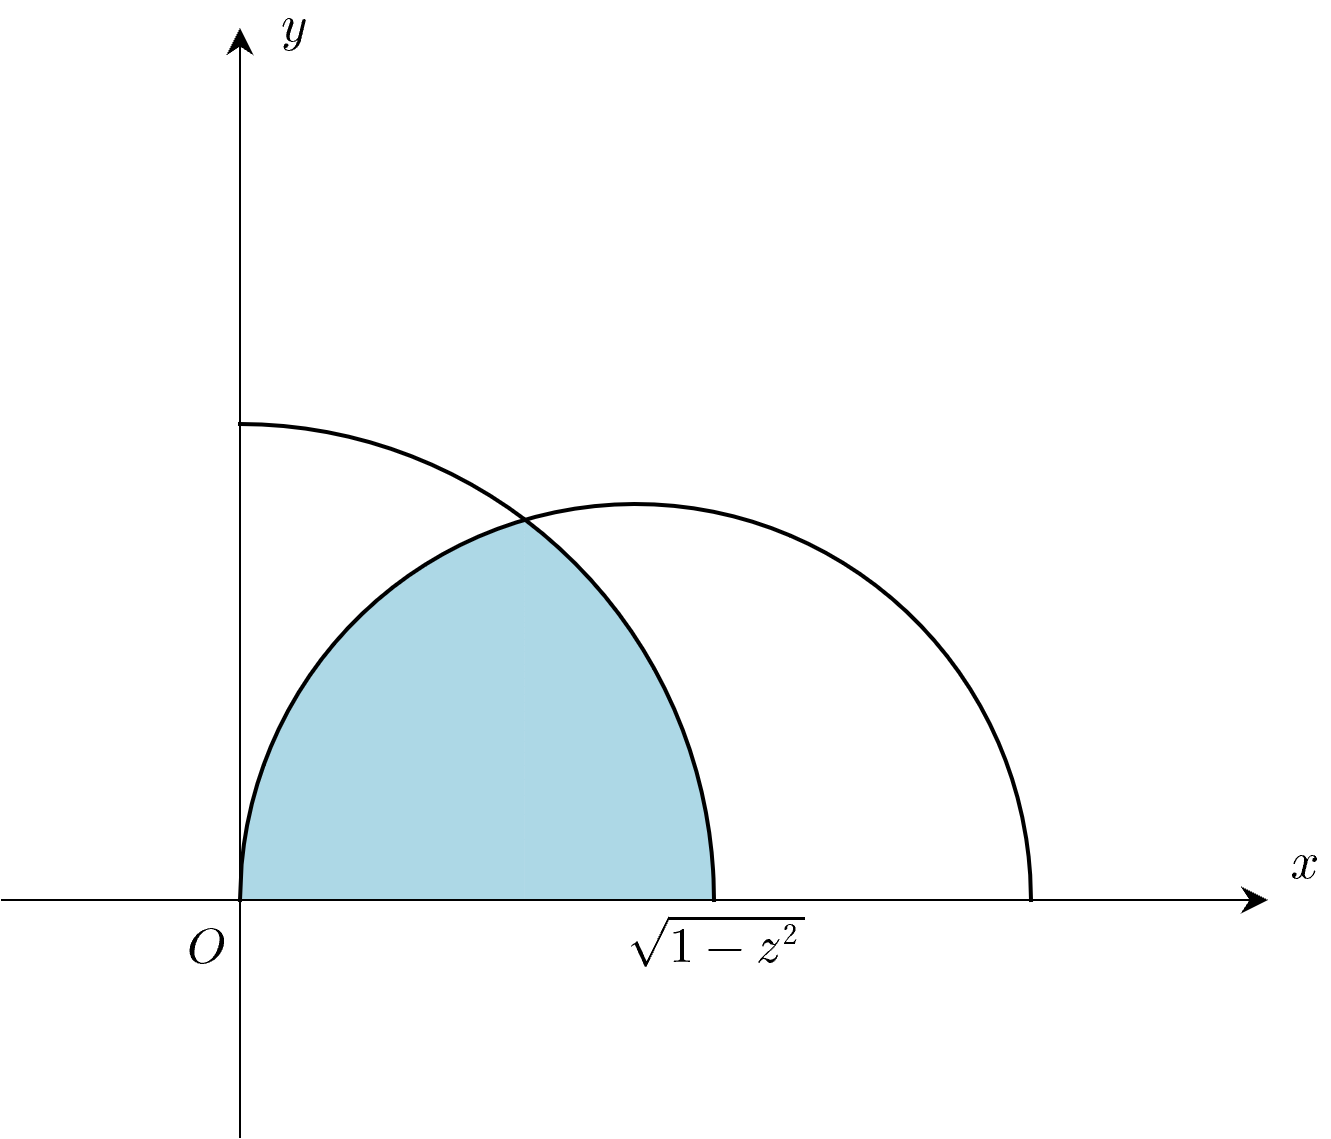
\includegraphics[width=.5\linewidth]{./src/fig/Basic/B_2021_spring_Dprime.png}
    \end{figure}
    % [] 積分領域 もう少し書く?
    求める体積$V$は
    \begin{align}
      V
      &= \iint_{D'} \sqrt{1-x^2-y^2}\,dxdy \\
      &= \int_{0}^{\pi/2}\int_{0}^{\cos\grt} r\sqrt{1-r^2}\,drd\grt \\
      &= \int_{0}^{\pi/2}d\grt \left[-\frac{1}{3}\bigl(1-r^2\bigr)^{3/2}\right]_{0}^{\cos\grt} \\
      &= -\frac{1}{3}\int_{0}^{\pi/2} \Bigl(\bigl(1-\cos^2\grt\bigr)^{3/2} - 1\Bigr) \,d\grt \\
      &= -\frac{1}{3}\int_{0}^{\pi/2} \bigl( \sin^3\grt - 1 \bigr)\,d\grt \\
      &= -\frac{1}{3}\left[ -\cos\grt + \frac{1}{3}\cos^3\grt - \grt \right]_{0}^{\pi/2} \\
      &= \frac{1}{3}\biggl(\frac{\pi}{2} - \frac{2}{3}\biggr)
    \end{align}
  \end{enumerate}
\end{ans*}


\prob{%
  次の微分方程式を解け。
  \begin{gather}
    (x+y)dx - (x-y)dy = 0
  \end{gather}
}
\begin{ans*}
  $x-y = 0$は$x+y=0$を得るので$y = x = 0$である。

  $x-y\neq 0$のとき、
  \begin{gather}
    \frac{dy}{dx} = \frac{x+y}{x-y}
  \end{gather}
  $x=0$のとき
    \begin{gather}
      \frac{dy}{dx} = -1\Rightarrow y = -x + C = C
    \end{gather}
  $x\neq 0$のとき、\dm{u = \frac{y}{x}}とおくと
  \begin{gather}
    \frac{dy}{dx} = \frac{du}{dx}x + u
  \end{gather}
  であるので、微分方程式は
  \begin{gather}
    \frac{du}{dx}x + u = \frac{1 + u}{1 - u} \\
    x\frac{du}{dx} = \frac{u^2 + 1}{1-u}
  \end{gather}
  とできる。変数分離形として
  両辺を積分して
  \begin{gather}
    \int\frac{1-u}{u^2+1}du = \int\frac{dx}{x} \\
    \arctan u - \frac{1}{2}\log(u^2+1) = \log |x| + C \\
    \arctan \frac{y}{x} - \frac{1}{2}\log\biggl(\frac{y^2}{x^2}+1\biggr) = \log |x| + C
  \end{gather}
\end{ans*}

\newpage
\subsection{線形代数}
\prob{
  正方行列\dm{
    \bA = \bmat{
      \disp\frac{9}{2} & \disp\frac{\sqrt{3}}{2} \\
      & \\
      \disp\frac{\sqrt{3}}{2} & \disp\frac{7}{2}
    }
  }について以下の問いに答えよ。

  \begin{enumerate}[label=\alph*)]
    \item $\bA$の固有値$\grl_1,\,\grl_2$\:($\grl_1>\grl_2$)と、
    それら固有値に対する単位長さの固有ベクトル
    \dm{\bn_1 = \Bmat{ n_{1x} \\n_{1y} }}
    \dm{\bn_2 = \Bmat{ n_{2x} \\n_{2y} }}
    を求めよ。
    \item 次の多項式を計算せよ。ただし、
    $\bI = \Bmat{ 1 & 0 \\ 0 & 1 }$である。
    \begin{gather}
      f(\bA) = \bA^5 - 6\bA^4 + 3\bA^3 - \bA^2 + 54\bA + 18\bI
    \end{gather}
  \end{enumerate}
}
\begin{ans*}
  ${}$
  \begin{enumerate}[label=\alph*)]
    \item 行列$\bA$の固有方程式より
    \begin{align}
      \biggl(\frac{9}{2} - \grl\biggr)\biggl(\frac{7}{2} - \grl\biggr) - \frac{3}{4}
      &= \grl^2 - 8\grl + 15 \\
      &= (\grl - 5)(\grl - 3) = 0 \\
    \end{align}
    \begin{gather}
      \therefore \grl = 5,\,3\:(=\grl_1,\,\grl_2)
    \end{gather}
    \begin{enumerate}[label=(\roman*)]
      \item $\grl = \grl_1$のとき、
      \begin{gather}
        \bA = \bmat{
          \disp -\frac{1}{2} & \disp\frac{\sqrt{3}}{2} \\
          & \\
          \disp\frac{\sqrt{3}}{2} & \disp -\frac{3}{2}
        }\Bmat{
          n_{1x} \\ n_{1y}
        }=\bzv \\
        \bn_1 = \frac{1}{2}\Bmat{
          \sqrt{3} \\ 1
        }
      \end{gather}
      \item $\grl = \grl_2$のとき、
      \begin{gather}
        \bA = \Bmat{
          \disp \frac{3}{2} & \disp\frac{\sqrt{3}}{2} \\
          & \\
          \disp \frac{\sqrt{3}}{2} & \disp \frac{1}{2}
        }\Bmat{
          n_{2x} \\ n_{2y}
        }=\bzv \\
        \bn_2 = \frac{1}{2}\Bmat{
          -1 \\ \sqrt{3}
        }
      \end{gather}
    \end{enumerate}
    \item 与えられた多項式は
    \begin{gather}
      f(\bA)
      = (\bA^2 - 8\bA + 15\bI)(\bA^3 + 2\bA + 4\bA + \bI) + 2\bA + 3\bI
    \end{gather}
    とできて、ケーリーハミルトンの定理より$\bA^2 - 8\bA + 15\bI=\bzv$から
    \begin{align}
      f(\bA)
      &= \bzv (\bA^3 + 2\bA + 4\bA + \bI) + 2\bA + 3\bI \\
      &= 2\bA + 3\bI \\
      &= \bmat{
        12 & \sqrt{3} \\
        \sqrt{3} & 10
      }
    \end{align}
  \end{enumerate}
\end{ans*}


\prob{
  \dm{
    \bD = \Bmat{ 1 & 4 \\ 2 & 5 \\ 3 & 6 },\,
    \bE = \Bmat{ 4 & 3 \\ 5 & 6 \\ 6 & 9 },\,
    \ba = \Bmat{ \gra \\ \beta \\ \grg },\,
    \bb = \Bmat{ \xi \\ \eta \\ \grk }
  }とする。\\
  いま、あるベクトル\dm{
    \bz = \Bmat{ p \\ q \\ r } \neq \bzv
  }が$\bD^{\top}\bz = \bzv$を満たしている。
  以下の問に答えよ。
  \begin{enumerate}[label=(\arabic*)]
    \item $p,\,q,\,r$の関係を示せ。
    \item $\bD\bx = \ba$の解\dm{
      \bx=\Bmat{ x_1 \\ x_2 }
      }が存在するとき、$\gra,\,\beta,\,\grg$が満たすべき必要条件を示せ。
    \item $\bE\by = \bb$の解\dm{
      \by=\Bmat{ y_1 \\ y_2 }
      }が存在するとき、$\gra,\,\beta,\,\grg$が満たすべき必要条件を示せ。
  \end{enumerate}
}

必要条件ではなく(必要)十分条件を問われているものと解釈しました。
必要条件なら適当に「$\ba\in\bbR^3$である」でもよい気がします。

また、(3)は$\gra,\,\beta,\,\grg$ではなく$\xi,\,\eta,\,\grk$の
条件を問われているものと解釈しました。

\begin{ans*}
  ${}$
  \begin{enumerate}[label=(\arabic*)]
    \item $\bD^{\top}\bz = \bzv$より
    \begin{gather}
      \bmat{
        1 & 2 & 3 \\
        4 & 5 & 6
      }\Bmat{
        p \\ q \\ r
      } = \bzv \\
      \begin{dcases*}
        p + 2q + 3r = 0 \\
        4p + 5q + 6r = 0
      \end{dcases*}
    \end{gather}
    \item $\bx$が解を持つためには$\rank \bD = \rank [\bD|\ba]$
    \begin{align}
      \bD
      &\lra \bmat{
        1 & 4 \\
        0 & -3 \\
        0 & 6
      } \\
      &\lra \bmat{
        1 & 4 \\
        0 & 1 \\
        0 & 0
      } \\
      &\lra \bmat{
        1 & 0 \\
        0 & 1 \\
        0 & 0
      } \\
      \therefore & \rank \bD = 2
    \end{align}
    また、
    \begin{align}
      \left[\begin{array}{cc|c}
        1 & 4 & \gra \\
        2 & 5 & \beta \\
        3 & 6 & \grg
      \end{array}\right]
      &\lra \left[\begin{array}{cc|c}
        1 & 4 & \gra \\
        0 & -3 & -2 \gra + \beta \\
        0 & -6 & -3 \gra + \grg
      \end{array}\right] \\
      &\lra \left[\begin{array}{cc|c}
        1 & 4 & \gra \\
        0 & -3 & -2 \gra + \beta \\
        0 & 0 & \gra - 2 \beta + \grg
      \end{array}\right] \\
      \therefore\rank[\bD|\ba]&=
      \begin{dcases*}
        2 & (\dm{\gra - 2 \beta + \grg = 0}) \\
        3 & (\dm{\gra - 2 \beta + \grg \neq 0})
      \end{dcases*}
    \end{align}
    ゆえに、解を持つ必要条件は\dm{\gra - 2 \beta + \grg = 0}

    \item $\by$が解を持つためには$\rank \bE = \rank [\bE|\bb]$
    \begin{align}
      \bE
      &\lra \bmat{
        4 & 3 \\
        5 & 6 \\
        6 & 9
      } \\
      &\lra \bmat{
        4 & 3 \\
        0 & \frac{9}{4} \\
        0 & \frac{9}{2}
      } \\
      &\lra \bmat{
        4 & 3 \\
        0 & \frac{9}{4} \\
        0 & 0
      } \\
      \therefore & \rank \bE = 2
    \end{align}
    また、
    \begin{align}
      \left[\begin{array}{cc|c}
        4 & 3 & \xi \\
        5 & 6 & \eta \\
        6 & 9 & \grk
      \end{array}\right]
      &\lra \left[\begin{array}{cc|c}
        4 & 3 & \xi \\
        &&\\
        0 & \disp\frac{9}{4} & \disp\frac{-5 \xi + 4\eta}{4} \\
        &&\\
        0 & \disp\frac{9}{2} & \disp\frac{-3 \xi + 2\grk}{2}
      \end{array}\right] \\
      &\lra \left[\begin{array}{cc|c}
        4 & 3 & \xi \\
        &&\\
        0 & \disp\frac{9}{4} & \disp\frac{-5 \xi + 4\eta}{4} \\
        &&\\
        0 & 0 & \xi - 2\eta + \grk
      \end{array}\right] \\
      \therefore\rank[\bE|\ba]&=
      \begin{dcases*}
        2 & (\dm{\xi - 2 \eta + \grk = 0}) \\
        3 & (\dm{\xi - 2 \eta + \grk \neq 0})
      \end{dcases*}
    \end{align}
    ゆえに、解を持つ必要条件は\dm{\xi - 2 \eta + \grk = 0}
  \end{enumerate}
\end{ans*}
